\documentclass{article}

\usepackage[english]{babel}
\usepackage[utf8]{inputenc}
\usepackage{fancyhdr}

\usepackage[a4paper, total={7in, 10in}]{geometry}
\usepackage{graphicx}

\graphicspath{ {./images/} }

\pagestyle{fancy}
\fancyhf{}
\fancyhead[L]{\leftmark}
\fancyhead[R]{\thepage}

% New commands
    \newcommand{\vect}[1]{\left[\begin{array}{c}#1\end{array}\right]}
    \newcommand{\ifcases}[1]{\left\{\begin{array}{cc}\end{array}\right.}
% 

\title{ETE Transistor}
\author{Samuel Nösslböck}
\date{April 2022}

\begin{document}

\maketitle

\section{Introduction}
    The known variables are
    \begin{equation}
        U_0 = 96V, \quad 
        R_{L} = 13.2\Omega, \quad 
        L = 60mH, \quad
        f_T = 1.5, 6, 24, 96 \textit{KHz}, \quad
        t_{TURN} = 12\mu s, \quad
        \frac{T_{OFF}}{T_{ON}} = 1.5
    \end{equation}

\section{PWM Signal}
    The bare PWM Signal has a Voltage over time graph depending on the frequency $f_T$ and the relation between active and inactive current flow.
    
    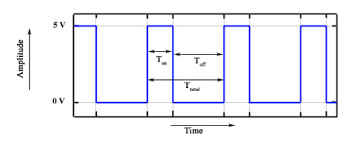
\includegraphics[]{images/PWM_Signal.png}
    
    The total time $T_{total}$ is calculated as follows
    \begin{equation}
        T_{total} = T_{ON} + T_{OFF} = \frac{1}{f_T} = \underline{666\mu s, 166\mu s, 41.6\mu s, 10.4\mu s}
    \end{equation}
    \begin{equation}
        T_{ON} = \frac{T_{total}}{2.5} \quad T_{OFF} = T_{total} - T_{ON}
    \end{equation}
    
    So the the variables for the four different frequencies result in
        \begin{center}
            \begin{tabular}{||c | c c c||} 
             \hline
             f_T & T_{total} & T_{ON} & T_{OFF} \\ [0.5ex] 
             \hline\hline
             1.5 & 666 \mu s & 266 & 400 \\ 
             \hline
             6 & 166 \mu s & 66.6 & 100 \\
             \hline
             24 & 41.6 \mu s & 16.7 & 25 \\
             \hline
             96 & 10.4 \mu s & 4.17 & 6.25 \\
             \hline
            \end{tabular}
        \end{center}
        
    \newpage
    
\section{Turn-Off sequence approximations}
    As the circuit has a given magnetism, the curves of voltage $u(t)$ and $i(t)$ are not vertical
    \begin{equation}
        u_{OFF}(t) = \frac{U_0}{2 \cdot t_P} \cdot t \cdot e^{-\frac{t}{2 \cdot t_P}} + U_0\cdot (1 - e^{\frac{-t}{T_{OFF}}});\quad t_P = \frac{T_{OFF}}{2}
    \end{equation}
    \begin{center}
        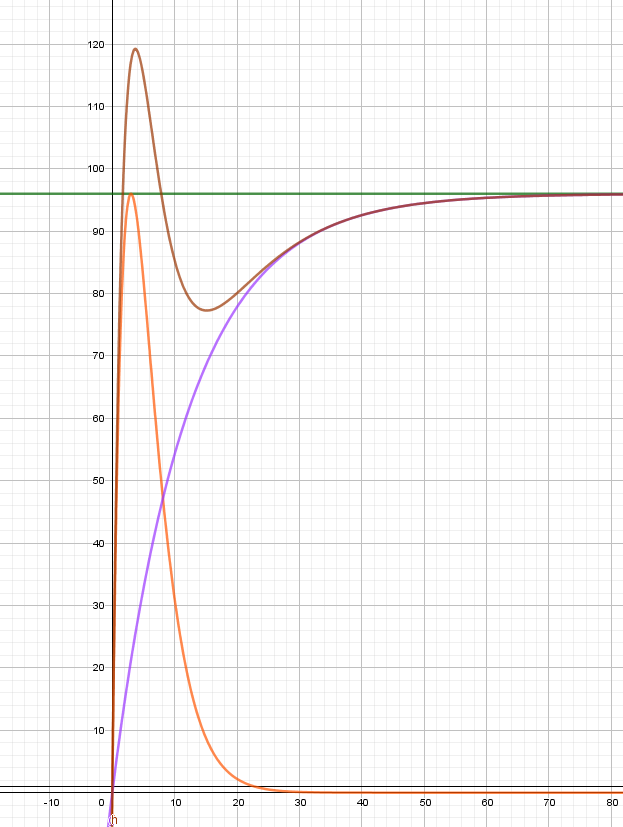
\includegraphics[scale=0.35]{images/VoltageApprox.PNG}
    \end{center}
    
    For the approximation of the current, the sigmoid function is used
    \begin{equation}
        i_{OFF}(t) = \frac{I_0}{1 + e^{\frac{x \ln(I_0)}{t_P/2}}}\quad t_P = \frac{T_{OFF}}{2}
    \end{equation}
    \begin{center}
        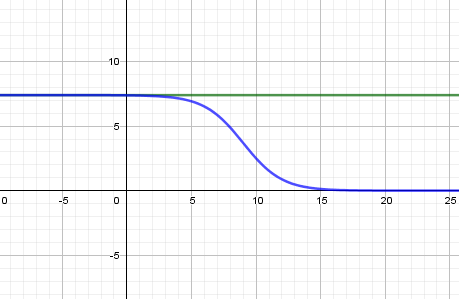
\includegraphics[scale=0.5]{images/CurrentApprox.PNG}
    \end{center}
    
    So the power is calculated using
    \begin{equation}
        p_{OFF}(t) = i_{OFF}(t) \cdot u_{OFF}(t)
    \end{equation}
    
    \begin{center}
        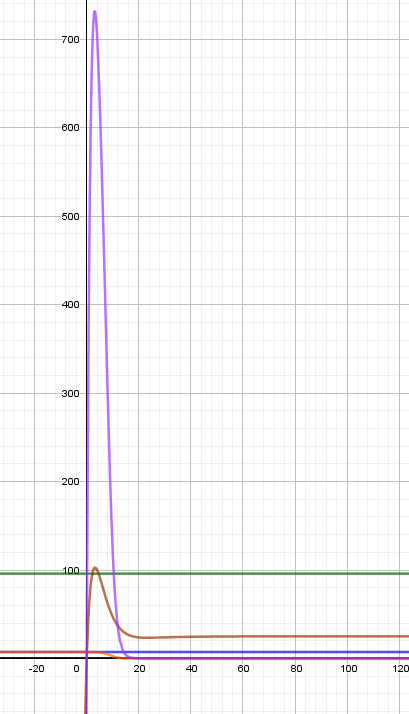
\includegraphics[scale=0.35]{images/PowerApprox.PNG}
    \end{center}
    
    \newpage
    
\section{Calculation}
    The actual calculation of the average power-usage is calculated as follows
    \begin{equation}
        I_0 = \frac{U_0}{R_L} = \underline{7.27A} \quad P_0 = I_0 \cdot 1V = \underline{7.27W}
    \end{equation}
    
    \begin{equation}
        \overline{P_{CE}} = \frac{ P_0 \cdot \Delta T_{OFF} + \overline{P_{OFF}} \cdot T_{TURN}}{\Delta t_{ON} + \Delta t_{OFF}};\quad \overline{P_{OFF}} = \frac{1}{T_{TURN}} \cdot \int_{0}^{ T_{TURN}} p_{OFF}(t)  dt 
    \end{equation}
    
    So the average power consumption for the four given frequencies
    
    \begin{center}
        \begin{tabular}{||c | c  c || } 
             \hline
             f_T & \overline{P_{OFF}} & \overline{P_{CE}} \\ [0.5ex] 
             \hline\hline
             1.5 & 400W & 11.6W  \\
             \hline
             6 & 400W & 33.1W \\
             \hline
             24 & 400W &  199.27W\\
             \hline
             96 & 400W & 465.9W\\
             \hline
        \end{tabular}
    \end{center}
    
    The last result does barley make sense, because the total period approaches the turn time
    
\section{Magnetism without diode}
    Without a diode, the energy of magnetism only passes out slowly. The energy of magnetism is calculated using
    \begin{equation}
        E_M = \frac{L \cdot I^2}{2}
    \end{equation}
    
    So an approximation would be
    \begin{equation}
        i(t) = I_0 \cdot e^\frac{-xR}{L}
    \end{equation}

    
\end{document}